% Prepared by Calvin Kent
%
% Assignment Template v19.02
%
%%% 20xx0x/MATHxxx/Crowdmark/Ax
%
\documentclass[12pt]{article} %
\usepackage{CKpreamble}
\usepackage{CKassignment}
\usepackage{tkz-euclide}
\usepackage{physunits}
\usepackage{physics}
\usepackage{lmodern}
\usepackage{microtype}
\usepackage{upgreek}
\usepackage{xcolor}
\usepackage{euscript}
\usepackage{tasks}
\usepackage{tkz-euclide}


\usepackage[misc]{ifsym}


%%Title
\title{Functions Quiz 2}
\date{January, 2022}

%%% Maths and science packages

\usepackage{amsmath,amsthm,amssymb}
\usepackage{pgfplots}
	\usetikzlibrary{
		calc,
		patterns,
		positioning
	}
	\pgfplotsset{
		compat=1.16,
		samples=200,
		clip=false,
		my axis style/.style={
			axis x line=middle,
			axis y line=middle,
			legend pos=outer north east,
			axis line style={
				->,
			},
			legend style={
				font=\footnotesize
			},
			label style={
				font=\footnotesize
			},
			tick label style={
				font=\footnotesize
			},
			xlabel style={
				at={
					(ticklabel* cs:1)
				},
				anchor=west,
				font=\footnotesize,
			},
			ylabel style={
				at={
					(ticklabel* cs:1)
				},
				anchor=west,
				font=\footnotesize,
			},
			xlabel= $x$,
			ylabel=$\vec d (\m \tx{[East]})$
		},
	}
	\tikzset{
		>=stealth
	}

%%% Tables and figures packages

\usepackage{float}
\usepackage{caption}
	\captionsetup{
		format=plain,
		labelfont=bf,
		font=small,
		justification=centering
	}
	
%%% Numbers and sets

\newcommand{\E}{\mathrm{e}}

\newcommand{\tx}[1]{\text{#1}}

\begin{document}
    \pagenumbering{arabic}
    % Start of class settings ...
    \renewcommand*{\coursecode}{MCR3U Quiz} % Quiz Title
    \renewcommand*{\assgnnumber}{2} % Quiz number
    \renewcommand*{\submdate}{January, 2022} % renew the date
    \renewcommand*{\studentfname}{\textbf{Name:}} % Student first name
    \renewcommand*{\studentlname}{} % Student last name
    %\renewcommand*{\studentnum}{SNumber} % Student number

    \renewcommand\qedsymbol{$\blacksquare$}
    \setfigpath
    % End of class settings 
    \pagestyle{crowdmark}
    \newgeometry{left=18mm, right=18mm, top=22mm, bottom=22mm} % page is set to default values
    \fancyhfoffset[L,O]{0pt} % header orientation fixed
    % End of class settings
    %%% Note to user:
    % CTRL + F <CHANGE ME:> (without the angular brackets) in CKpreamble to specify graphics paths accordingly.
    % The command \circled[]{} accepts one optional and one mandatory argument.
    % Optional argument is for the size of the circle and mandatory argument is for its contents.
    % \circled{A} produces circled A, with size drawn for letter A. \circled[TT]{A} produces circled A with size drawn for TT.
    % https://github.com/CalvinKent/My-LaTeX
    %%%
    % Crowdmark assignment start


    %%%%%%%%%%%%%%%%%%%%%%%%%%%%%%%%%%%%%%%%%%%%%%%%%%%%%%%%%%%%%%%%%%%%%%%%%%%%%%%%%%%%%%%%%%%%%%%%%%%%%%%%
    %%%%%%%%%%%%%%%%%                  PROBLEM IDEAS                  %%%%%%%%%%%%%%%%%%%%%%%%%%%%%%%%%%%%%%
    %%%%%                   ----------------------------------------                                %%%%%%%%

    % --> Do a hard tangent line problem

	\maketitle
\section{Name and Date:}
	Print your name and todays date below;\\


	\begin{center}
	\noindent\begin{tabular}{ll}
		\makebox[3in]{\hrulefill} & \makebox[3in]{\hrulefill}\\
		Name & Date\\[8ex]% adds space between the two sets of signatures
	\end{tabular}
	\end{center}
	\newpage


\begin{qstn}[1][(8 points)] % qnumber, qname, qpoints
  Answer the following True/False questions,
  \begin{enumerate}
    \item Let $\operatorname{id}_\R \colon \R \to \R$ be the identity function on $\R$, then
       \[
              \operatorname{id}_\R\left(\operatorname{id}_\R\left(\operatorname{id}_\R\left(\operatorname{id}_\R\left(\operatorname{id}_\R\left(\operatorname{id}_\R\left(2
              \right) \right) \right) \right) \right) \right) = 2
      .\] 
      Circle the correct answer: \,\, \textbf{True} \,\,\,\,\,\, \textbf{False}

    \item Let $\phi \colon \mathcal{A} \to \mathcal{B}$ be an $\textit{injective}$ function, then every element in
      $\mathcal{B}$ is mapped to.\\
          Circle the correct answer: \,\, \textbf{True} \,\,\,\,\,\, \textbf{False}

    \item Let $\mathcal{L} \colon \mathcal{A} \to \mathcal{B}$ be a $\textit{surjective}$ function, then
          $\left|\mathcal{R_\mathcal{L}}\right| = \left|\mathcal{B}\right|$, where $\mathcal{R_\mathcal{L}}$ is the
          range of $\mathcal{L}$.\\
          Circle the correct answer: \,\, \textbf{True} \,\,\,\,\,\, \textbf{False}

    \item Let $\lambda \colon \mathcal{A} \to \mathcal{B}$ be a function, suppose $\lambda$ is one of surjective or
      injective, then $\lambda$ is invertible.\\
          Circle the correct answer: \,\, \textbf{True} \,\,\,\,\,\, \textbf{False}

    \item Let $ \mathcal{X} = \{-1,0,1\} $ and $ \mathcal{Y} = \{-1,1,2\} $ be sets, lets define the
            following function, 
            \begin{itemize}
              \item $\mathcal{\eta} \colon \mathcal{X} \to \mathcal{Y}$.
              \item $\mathcal{\eta}(x) = 2x^2 - 1$.
            \end{itemize}
            Then $\eta$ is an invertible function.\\
          Circle the correct answer: \,\, \textbf{True} \,\,\,\,\,\, \textbf{False}
   \item Let $ \mathcal{V} = \{-2,0\} $ and $ \mathcal{W} = \{0,4\} $ be sets, 
              define the following function, 
              \begin{itemize}
                \item $\mathcal{T} \colon \mathcal{V} \to \mathcal{W}$.
                \item $\mathcal{T}(v) = v^2$.
              \end{itemize}
              Then the function,
              \begin{itemize}
                \item $\mathcal{T}^{-1} \colon \mathcal{W} \to \mathcal{V}$.
                \item $\mathcal{T}^{-1}(w) = \sqrt{w}$.
              \end{itemize}
              is the inverse function for $\mathcal{T}$.\\
      Circle the correct answer: \,\, \textbf{True} \,\,\,\,\,\, \textbf{False}


   \item Let $\textbf{A}$ and $\textbf{B}$ be binary strings, then $\textbf{A} + \textbf{B} = \textbf{B} +
        \textbf{A}$.\\
      Circle the correct answer: \,\, \textbf{True} \,\,\,\,\,\, \textbf{False}

    \item Let $G \colon \mathcal{H} \to \mathcal{T}$ be a function. If 
      $\left|\mathcal{H}\right| = \left|\mathcal{T}\right|$, then $G$ is invertible.\\
      Circle the correct answer: \,\, \textbf{True} \,\,\,\,\,\, \textbf{False}

  \end{enumerate}
\end{qstn}



\begin{qstn}[2][(8 points)]
  For each of the following, you are given a function and its definition. For each question,
  \begin{itemize}
    \item Prove that the function is invertible \textbf{or} prove that the function is not invertible.
    \item Determine the range of the function.
  \end{itemize}
  \begin{enumerate}[label=(\alph*)]
    \item $g \colon \mathcal{A} \to \mathcal{B}$,
    \begin{center}
     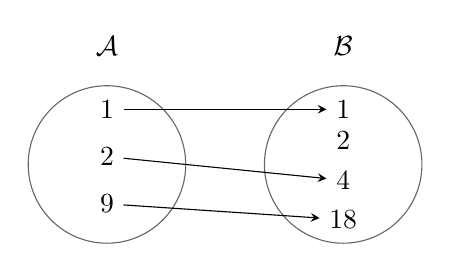
\begin{tikzpicture}
        % draw the sets
        \filldraw[fill=white!20, draw=black!60] (-1.5,0) circle (1cm);
        \filldraw[fill=white!20, draw=black!60] (1.5,0) circle (1cm);


        % the texts
        \node at (-1.5,1.5) {$\mathcal{A}$};
        \node at (1.5,1.5) {$\mathcal{B}$};

        % the points in the sets (here I just create nodes to use them later on to position
        % the circles and the arrows
        \node (x1) at (-1.5,0.7) {$1$};
        \node (x2) at (-1.5,0.1) {$2$};
        \node (x4) at (-1.5,-0.5) {$9$};
        \node (y1) at (1.5,0.7) {$1$};
        \node (y2) at (1.5,0.3) {$2$};
        \node (y3) at (1.5,-0.2) {$4$};
        \node (y4) at (1.5,-0.7) {$18$};

        % draw the arrows
        \draw[->] (x1) -- (y1);
        \draw[->] (x2) -- (y3);
        \draw[->] (x4) -- (y4);

    \end{tikzpicture}
  \end{center}


    \vspace*{5cm}



  \item Let $\mathcal{X} = \{-3-2,0,1\} $, $\mathcal{Y} = \{0,1,2,3\}$ be sets and define,
    \begin{itemize}
      \item $H \colon \mathcal{X} \to \mathcal{Y}$.
      \item $H(x) = \left|x\right|$.
    \end{itemize}
  \end{enumerate}
\end{qstn}



\begin{qstn}[3][(7 marks)]
Let $ \mathcal{X} = \{3,7,4\} $ and $ \mathcal{Y} = \{2,0,1\} $ be sets, define the following function, 
\begin{itemize}
    \item $A \colon \mathcal{X} \to \mathcal{Y}$.
    \item $A(x) = \sqrt{x - 3}$.
\end{itemize}
Prove that the function,
\begin{itemize}
    \item $A^{-1} \colon \mathcal{Y} \to \mathcal{X}$.
    \item $A^{-1}(y) = y^2 + 3$.
\end{itemize}
is the inverse function for $\mathcal{L}$. \\
\textbf{Hint:} Use mapping tables.
  
\end{qstn}

\begin{qstn}[4][(3 marks)]
Let $\EuScript{S} = \{101,010,111\}$  and $\EuScript{R} = \{11,01,10\}$ be sets of binary strings, define the following function,
\begin{itemize}
    \item $Q \colon \EuScript{S} \to \EuScript{R}$.
    \item $Q(\textbf{S}) = \vb s_1 \vb s_2$.
\end{itemize}
Prove that the function,
\begin{itemize}
    \item $Q^{-1} \colon \EuScript{R} \to \EuScript{S}$.
    \item $Q^{-1}(\textbf{R}) = \textbf{R} + 1$.
\end{itemize}
is \textbf{NOT }the inverse function for $Q$.\\
\textbf{Hint:} Which of the two conditions in Definition 4.1 does it fail to preserve?

  
\end{qstn}
































\end{document}
